\documentclass[a4paper,12pt]{scrreprt}                       % default is A4 paper style and 11pt font size


%%%%%%%%%%%% version history %%%%%%%%%%%%%%%%%%%%%%%%%%%%%%%%%%%
%27.05.2021: updates about layout/plagiarism from Monica Patrascu, Bogdan Dumitrescu
%25.04.2020:  modified the lst definitions (monospaced, gray); localized versions (romanian) for the \autoref command; updated the romanian.lbx file
%26.03.2017:    corrections for the latex source-code: diacritics issues; corrected the glossaries and added listings packages; added fontspec (only works with xelatex/lualatex !!!)
%2014:          put in latex version + some small additions - Florin Stoican
%2013:          content from Dan Stefanoiu
%%%%%%%%%%%%%%%%%%%%%%%%%%%%%%%%%%%%%%%%%%%%%%%%%%%%%%%%%%%%%%%%%%%%%%%%%


%%%%%%%%%%%% macros for various paths %%%%%%%%%%%%%%%%%%%%%%%%%%%%%%%%%%%
\def \cls {./cls}                                            % path to common latex files (change for your own relative/absolute path)
\def \pics {./img}                                          % path to pics files (change for your own relative/absolute path)
\def \chapters {./tex}                                  % path to chapter files (change for your own relative/absolute path)
\def \code {./code}                                          % path to source code files (change for your own relative/absolute path)

% you don't have to use them but it's nicer this way
%%%%%%%%%%%%%%%%%%%%%%%%%%%%%%%%%%%%%%%%%%%%%%%%%%%%%%%%%%%%%%%%%%%%%%%%%

% language={english/romanian} selects between the languages used in the manusript (changes, e.g., the name of the chapter)
% type={bachelor/master/phd} selects between the type of manusript (changes, e.g., the titlepage make-up)
\usepackage[language=romanian,type=bachelor]{\cls/standard} % introduces useful packages and commands(CHANGE ONLY IF YOU KNOW WHAT YOU'RE DOING)
\addbibresource{references.bib}                             % bib resource (using biblatex package, for complex stuff use the biber backend instead of bibtex
% \include{\cls/gls}                                          % put here all your glossary terms; only the ones actually used will appear in the glossary list of the manuscript

\newacronym{io}{IO}{Input/Output}
\newacronym{ip}{IP}{Internet Protocol}
\newacronym{fp}{FP}{Functional Programming}
\newacronym{tht}{THT}{Through Hole Technology}
\newacronym{smd}{SMD}{Surface Mounted Device}
\newacronym{hat}{HAT}{Hardware attached on top}
\newacronym{frp}{FRP}{Functional Reactive Programming}
\newacronym{cad}{CAD}{Computer Assisted Design}
\newacronym{dto}{DTO}{Data Transfer Object}
\newacronym{oop}{OOP}{Object Oriented Programming}
\newacronym{iot}{IoT}{Internet of Things}
\newacronym{ssl}{SSL}{Secure Sockets Layer}
\newacronym{aws}{AWS}{Amazon Web Services}
\newacronym{api}{API}{Application Programming Interface}
\newacronym{adc}{ADC}{Analog to Digital Convertor}
\newacronym{dac}{DAC}{Digital to Analog Convertor}
\newacronym{gsm}{GSM}{Global System for Mobile Communications}
\newacronym{sim}{SIM}{Subscriber Identity Module}
\newacronym{pcb}{PCB}{Printed Circuit Board}
\newacronym{osi}{OSI}{Open Systems Interconnection}
\newacronym{mvc}{MVC}{Model View Controller}
\newacronym{jwt}{JWT}{JSON Web Token}
\newacronym{napi}{N-API}{Node-API}
\newacronym{dtmf}{DTMF}{Dual-Tone Multi-Frequency}
\newacronym{json}{JSON}{JavaScript Object Notation}
\newacronym{gpio}{GPIO}{General-Purpose Input/Output}
\newacronym{voip}{VoIP}{Voice Over IP}
\newacronym{pots}{POTS}{Plain Old Telephone Service}
\newacronym{rest}{REST}{Representational State Transfer}
\newacronym{rfid}{RFID}{Radio-Frequency Identification}
\newacronym{mosfet}{MOSFET}{Metal Oxide Semiconductor Field Effect Transistor}
\newacronym{arpanet}{ARPANet}{Advanced Research Projects Agency Network}
\newacronym{hmac}{HMAC}{Hash-Based Message Authentication Codes}
\newacronym{sha256}{SHA-256}{Secure Hash Algorithm 256 biti}
\newacronym{hs256}{HS256}{HMAC SHA-256}


\begin{document}

%%%%%%%%%%%%%%%%%%%%%%% frontmatter %%%%%%%%%%%%%%%%%%%%%%%%%%%%%%%%%%%%%
\pagenumbering{roman}                                       % default numbering for the frontmatter is roman

\title{Sistem IoT pentru controlul\\accesului \^{i}n clădire}
\author{Alexandru Cristian IONESCU}
\advisor{Mihnea Alexandru MOISESCU}

\maketitle

% show table of contents, figures, tables and algorithms

\tableofcontents 
\printglossaries                                       % \printglossaries works only if the makeindex has the correct arguments
\listoffigures 
\addcontentsline{toc}{chapter}{\listfigurename}
\listoftables
\addcontentsline{toc}{chapter}{\listtablename}
\listofalgorithmes
\addcontentsline{toc}{chapter}{\listalgorithmcfname}

\clearpage

%%%%%%%%%%%%%%%%%%%%%%% mainmatter %%%%%%%%%%%%%%%%%%%%%%%%%%%%%%%%%%%%%%
\pagenumbering{arabic}                                      % default numbering for the mainmatter is arabic

% here is the text of you manuscript; you can put it directly here but it is better to include files (the main file will be more compact)
\chapter{Introducere}
\section {Obiectivele lucrării de licența}

\subsection {Realizarea unui studiu de piata pentru determinarea fezabilitatii solutiei}

In continuare voi realiza un scurt studiu de piata pe nisa sistemelor \acrfull{iot} destinate uzului casnic. Un caz particular de astfel de dispozitive sunt cele care indeplinesc functia de interfon sau ofera contrulul accesului intr-o incinta de la distanta.

In momentul de fata exista pe piata o multitudine de produse de tip incuietoare inteligenta sau sisteme tip interfon GSM, atat de la producatori cunoscuti cat si de la branduri nou infiintate. Aceasta lucrare va analiza trei tipuri de solutii existente, cu implementari diferite, incercand sa identifice functionalitati comune, avantaje si dezvantaje dintr-o plaja cat mai mare de dispozitive.

Solutiile prezentate mai sus au dezavantaljul ca nu au fost concepute sa fie integrate cu un sistem existent, intr-un bloc mai vechi. Prin urmare exista un segment de piata de utilizatori care ar dori sa benefecieze de functiile intefonului inteligent, dar nu pot deoarece asta ar presupune schimbarea sistemului din intreaga cladire.


\subsection {Dezvoltarea unui sistem compatibil POTS pentru interfatarea in reteaua IoT}

Pentru a putea oferi functiile inteligente unei audiente cat mai large, sistemul propus in aceasta lucrare se poate conecta la reteaua \acrfull{pots} printr-o simpla mufa RJ11.


\section {Descrierea domeniului din care face parte tema de licența}

Aceasta lucrare face parte dintr-un domeniu mai vechi, dar care a prins amploare recent, domeniul automatizarilor casnice si IoT. 


\subsection {Istoric}

Interesul in conectarea locuintelor pentru a obtine functionalitate aditionala dateaza inca din anii 60, majoritatea fiind concepte prototipate de entuziasti cu inclinatii spre electronica.

Jim Sutherland, inginer la Westinghouse a creat primul sistem de automatizare a domiciliului in anul 1964, ECHO IV. Acesta era capabil sa controleze temperatura, alte aparate casnice cat si sa permita retinerea de mementouri sau liste de cumparaturi. Cu introducerea retelei \acrfull{arpanet} in 1969, un precursor al Internetului, universul dispozitivelor casnice conectate a cunoscut o perioada rapida de dezvoltare in anii urmatori \cite{ZeusIntegratedSystems}.

Trecerea de la o noutate scumpa la un sistem ce ofera functii cu adevarat practice a venit sub forma proiectului "X10 Home Automation". Acesata se putea integra cu sistemul de climatizare existent al cladirii, controla electrocasnice mici, cat si corpuri de iluminat.

In anul 1984, Asociatia Nationala a Constructorilor din Statele Unite a creat un grup de control numit "Smart House" pentru a accelera includerea tehnologiei in proiectele viitoare \cite{Aldrich2003Smart}.

Pentru consumatori, dezvoltarile din urmatorii ani au adus usi automate pentru garaje, termostate programabile si sisteme de securitate in cadrul monden, concomitent reducand preturile solutiilor oferite. In ciuda acestor semne, sociologii au concluzionat la vremea respectiva ca nu exista un interes real in conceptul "Smart House".


\subsection {Stadiu actual}

Solutiile de tip "Smart Home" din prezent se integreaza in general cu o retea precum Espressif, Apple HomeKit sau Google Home. Aceasta permite controlul dispozitvelor conectate prin intermediul telefonului mobil.

\href{https://www.familyhandyman.com/article/the-history-of-smart-home-technology/}{Apple HomeKit/Google Home}

\href{https://techcrunch.com/2013/05/11/from-the-garage-to-200-employees-in-3-years-how-nest-thermostats-were-born/}{Nest TC}


\section {Prezentare pe scurt a capitolelor}

//To do

\chapter{Descrierea problemei abordate}
\section {Formularea problemei}

In orase precum Bucuresti, majoritatea blocurilor au fost contruite inainte de anul 1990 si prin urmare interfoanele lor se bazeaza pe \acrshort{pots}. Traind in era digitala, utilizatorul ideal (e corporatist) isi doreste augmentarea functionalitatilor sistemului existent, pentru a nu trebui sa isi convinga toti vecinii sa investeasca in modernizarea sistemului de acces. Pentru a putea adresa cat mai multi utilizatori, solutia acestei probleme trebuie sa fie agnostica de smartphoneul si interfonul existent a utilizatorului, dar sa ofere integrari cu alte solutii de tip "Smart Home".

In functie de perioada instalarii, sistemele sa impart in doua categorii: analogice si digitale. Posturile de interfon analogice sunt legate la o unitate de comanda care decodeaza semnale \acrfull{dtmf}, genereaza un semnal sinusoidal cu frecventa de 20Hz si amplitudinea de 60-90V pentru sonerie, apoi realizeaza conexiunile necesare dintre postul de afara si cel al apartamentului cautat. Sistemele digitale folosesc o magistrala comuna de comunicatii, fiind adresate conform unei scheme prestabilite - fiecare terminal este programat cu o adresa, insa pentru acest procedeu este nevoie de o cheie asociata unitatii de comanda.

Din motive istorice, unitatea centrala \acrshort{pots} genereaza semnalul sinusoidal si poarta suficient curent pentru a putea alimenta clopotul aparut in prima generatie de telefoane. Prin urmare, sistemele digitale sunt considerate mai eficiente si mai sigure, dar si mai greu de integrat, datorita implicarii unei persoane autorizate care sa programeze intregul sistem.

Aceasta lucrare va analiza solutii digitale, insa sistemul final va fi implementat pe un terminal analog. Asadar, trebuie sa intelegem in primul rand mecanismul de adresare si cum este el interpretat de centrala. Dupa cum insinueaza numele, \acrshort{dtmf} presupune generarea a doua tonuri de frecevente diferite in acelasi timp, conform liniei si coloanei tastei apasate. Acest semnal va fi intrepretat de decodorul de semnal al centralei cu ajutorul unor filtre de tip notch spre a se realiza conexiunile necesare. 

\begin{table}[ht!]
\begin{tabular}{c||c|c|c}
 & 1209Hz & 1336Hz & 1477Hz \\
\hline
\hline
697Hz & 1 & 2 & 3 \\
\hline
770Hz & 4 & 5 & 6 \\
\hline
852Hz & 7 & 8 & 9 \\
\hline
941Hz & * & 0 & \# \\
\end{tabular}
\centering
\caption{Tabel frecvente \acrshort{dtmf}}
\label{tab:dtmf}
\end{table}

Sistemul descris pana acum poate adresa $12-1=11$ posturi diferite (centrala este considerata si ea post si are un slot rezervat). Pentru a adresa mai multe posturi, unitatea de comanda trebuie sa includa si un circuit logic secvential pentru a retine starea ultimelor taste apasate. Astfel, ajungem la un numar satisfacator de adrese pentru aplicatia interfonului. 

Un exemplu de analiza spectrala a unui astfel de semnal:

\begin{figure}[h!]
  \centering
  \fbox {
    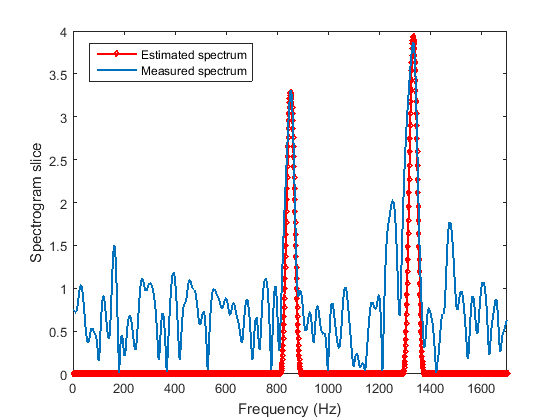
\includegraphics[width=\singlefigure]{02/04_spectru_dtmf.png}  
  }
  \caption{Spectrograma tasta "8" \cite{AunsriNattapol2016}}
\end{figure}

Se pot distinge grafic doua frecvente predominante: 852Hz si 1336Hz - cobinatia corespunaztoare tastei "8".

\section {Studiu asupra realizărilor similare din domeniu}


\subsection {Videx UK}

Interfoanele \acrshort{gsm} de la Videx sunt conectate la reteaua mobila de telefonie si permit operarea unei porti prin intermediul unui releu. Ele necesita doar o sursa de curent externa, o antena si o cartela \acrfull{sim} pentru a opera.

\begin{figure}[h!]
  \centering
  \fbox {
    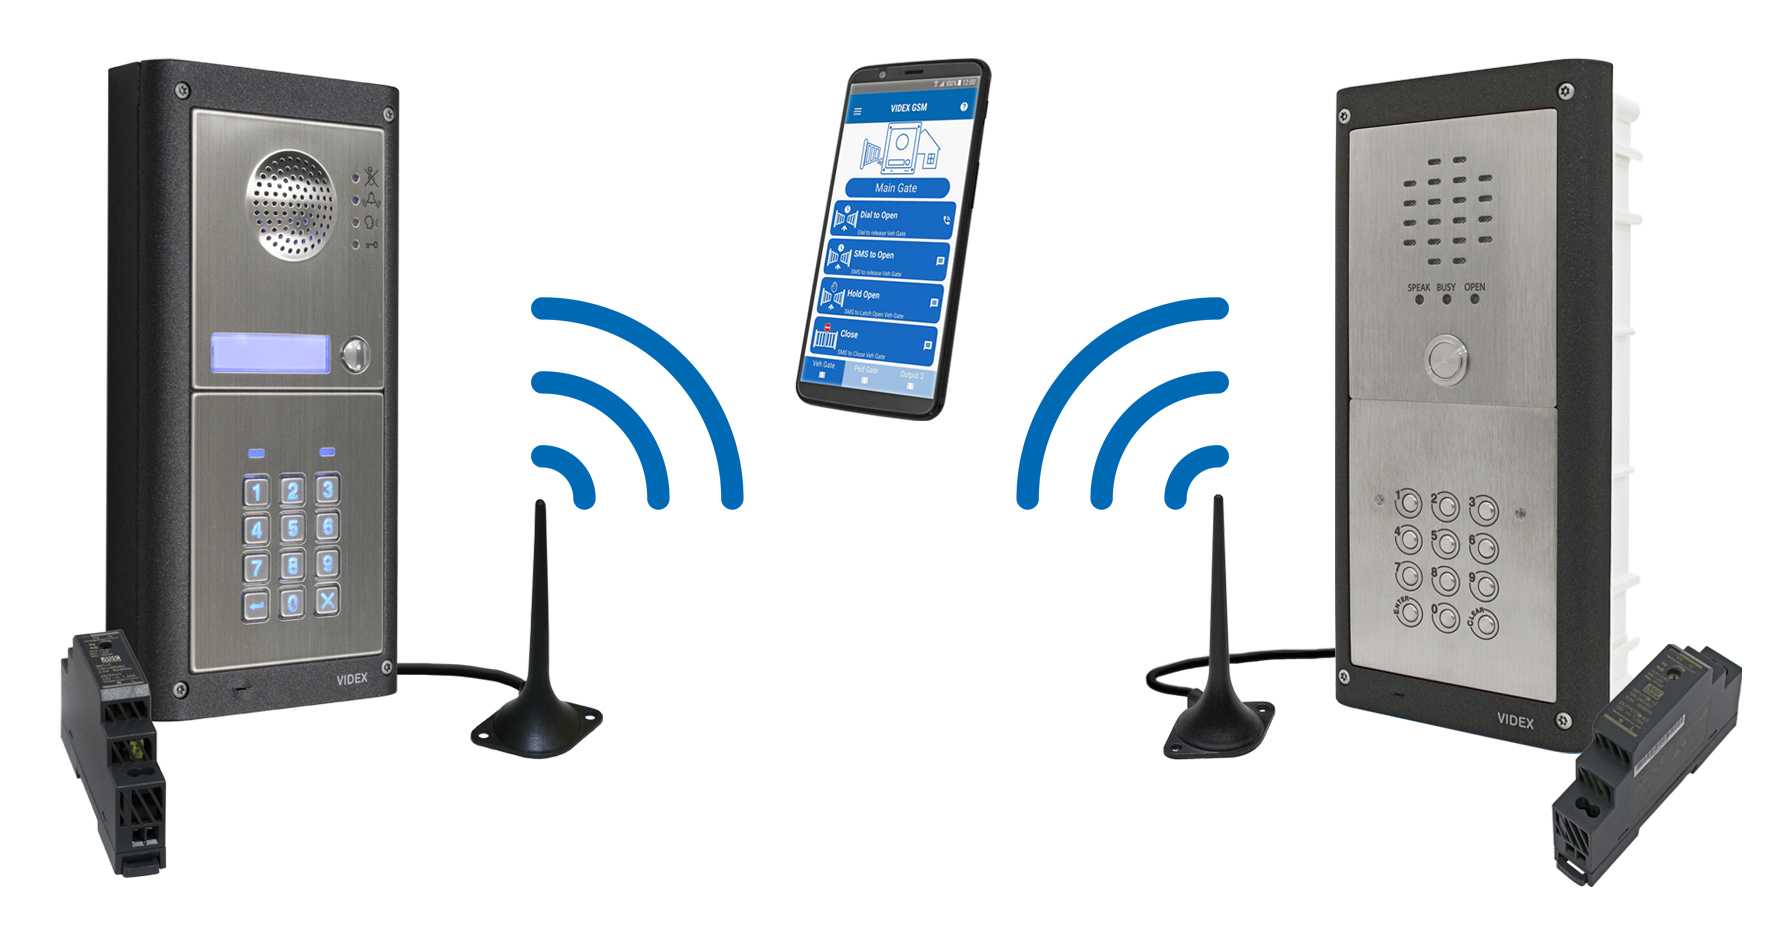
\includegraphics[width=\singlephoto]{02/01_gsm_system.jpg}  
  }
  \caption{Sistem interfon Videx GSM \cite{VidexUk}}
\end{figure}

Printre functionalitatile principale se numara:
\begin{itemize}
  \item Poate include un cititor de carduri \acrshort{rfid} si cheie
  \item Versiune rezistenta la vandalism
  \item Pana la 4 numere de telefon per apartament, pentru redundanta. In cazul in care primul numar nu se poate apela sau nu raspunde, se va incerca urmatorul numar programat
  \item Ofera aplicatie Android si iOS pentru programat unitatea
\end{itemize}

Dezavantaje:

\begin{itemize}
  \item Nu ofera integrare cu servicii din reteaua \acrshort{iot}
\end{itemize}

\subsection {Google Nest x Yale Lock}

\begin{figure}[h!]
  \centering
  \fbox {
    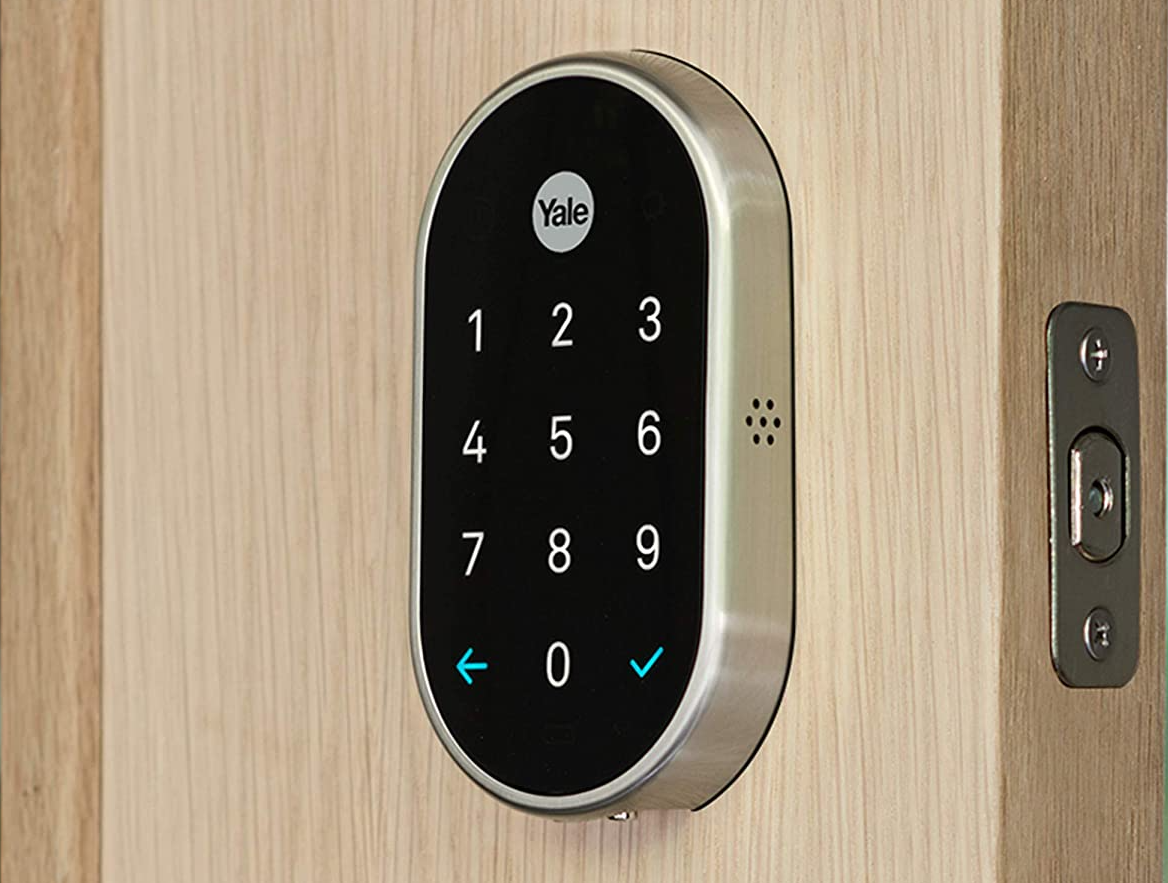
\includegraphics[width=\singlephoto]{02/02_iot_system.png}  
  }
  \caption{Next x Yale Lock \cite{YaleLock}}
\end{figure}

Avantaje:
\begin{itemize}
  \item Permite accesul prin intermediul unui PIN ales de utilizator
  \item Ofera alerte cand cineva inchide sau deschide usa
  \item Ofera integrare cu Google Home si Nest Home
\end{itemize}

Dezavantaje:
\begin{itemize}
  \item Are nevoie de 4 baterii tip AA pentru a functiona
  \item Nu are acces cu cheie sau cartela
  \item Nu are versiune rezistenta
\end{itemize}


\subsection {Level Lock - Touch Edition}

Level Lock este o incuietoare inteligenta de tip zavor. Are un design minimalist si ascunde partea electronica in interiorul usii pentru mai multa securitate.

\begin{figure}[h!]
  \centering
  \fbox {
    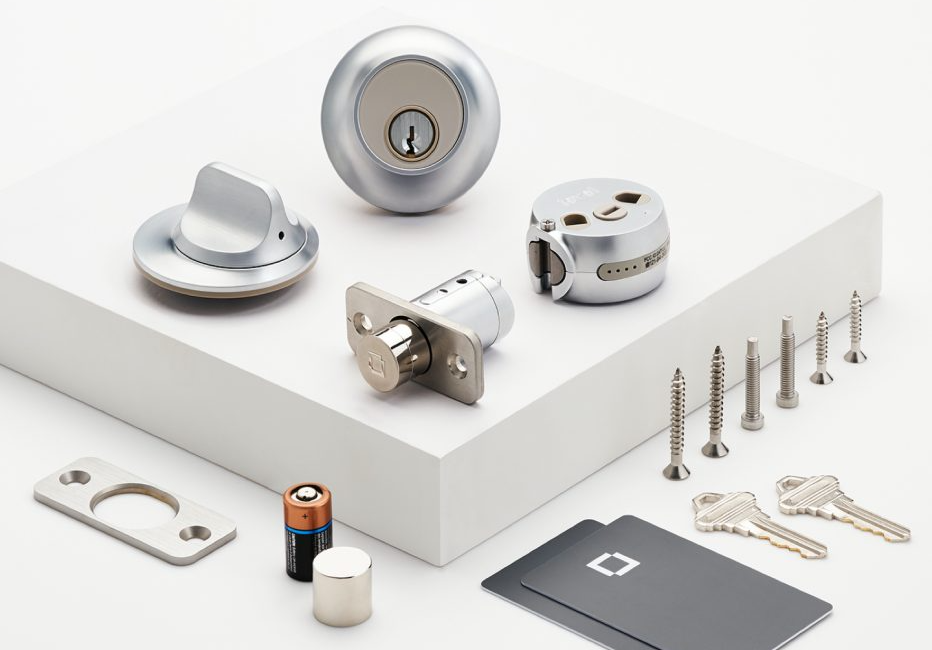
\includegraphics[width=\singlephoto]{02/03_iot_system.jpg}  
  }
  \caption{Level Lock \cite{LevelLock}}
\end{figure}

Avantaje:
\begin{itemize}
  \item Multiple modalitati de acces, printre care: amprenta, PIN
  \item Ofera alerte cand cineva inchide sau deschide usa
  \item Ofera integrare cu Google Home si Nest Home
\end{itemize}

\subsection {Comparatii}

Produsele de mai sus adreseaza probleme usor diferite, dar incearca sa ofere functionalitati similare. Sistemul oferit de Videx Security prezinta un design rezistent, dar familiar tuturor utilizatorilor si este destinat cladirilor cu mai multi locatari. In contrast, cele doua incuietori inteligente ofera o integrare avansata in reteaua \acrshort{iot} si multiple cai de acces, dar sunt destinate unei singure locuinte.

Incuietoarea de la Yale prezinta cea mai inovativa abordare a acestul design prin decizia deliberata de a nu oferi posibilitatea de acces cu cheie. Astfel, simplifica partea mecanica eliminand singura cale de acces din exterior catre mecanismul incuietorii.

Produsul celor de la Videx Security se bazeaza pe o tehnologie utilizata la scara larga si prin urmare beneficiaza de robustetea unui sistem matur. Spre deosebire de celelalte doua produse analizate, solutia celor de la Videx Security este agnostica de sistemul de operare al telefonului mobil, avand nevoie doar de o conexiune \acrshort{gsm}.

Din lipsa unor standarde in domeniu, dispozitivele noi sufera de alte tipuri de probleme si vulnerabilitati, dupa un studiu realizat de cercetatorii de la Bitdefender. Majoritatea sunt in faza initiala de setare, oferind protocoale de securitate invechite sau omitandu-le complet. Este mentionat si un dispozitiv care expune un port Telnet, un protocol invechit si usor de exploatat, fara posibilitatea de a fi dezactivat \cite{Bitdefender2016IoT}.

\section {Stabilirea cerințelor funcționale si nefuncționale ale sistemului}
// todo: impartit in functionale/nefunctionale

\subsection{Controlul accesului intr-un apartament}

Scopul principal al acestui sistem este de a oferi sau nu acces intr-o incinta, prin urmare consider aceasta cea mai importanta cerinta functionala.

\subsection{Expunerea unui serviciu REST pentru interfatarea cu alte sisteme}

Expunerea si abstractizarea terminalului \acrshort{pots} este realizata printr-un set de servicii \acrfull{rest} care controleaza starea sa. Acest lucru ne permite interfatarea cu aplicatia mobila, interfata de administrare web si alte servicii precum Google Home/Google Assistant/Apple HomeKit.

\subsection{Implementarea unei functii pentru raspuns automat}

Aceasta functie va permite utilizatorului sa stabileasca o perioada de timp pentru care sistemul va oferi accesul neconditionat.

\subsection{Dezvoltarea unui client mobil Android}

Principalul client care va interactiona cu serviciile \acrshort{rest} va fi aplicatia mobila ce va avea rolul de a notifica userul cand ii suna interfonul si de a controla starea sistemului.

\subsection{Control granular asupra datelor stocate}

Arhitectura aplicatiei necesita interactiunea cu o baza de date, care poate fi tinuta in cloud, pentru convenabilitate sau local.
Folosind tehnologii de containerizare precum Docker, putem stoca baza de date local, informatiile fiind stocate intr-un mediu controlat.

\subsection{Criptarea comunicatiilor cu serviciile web}

Avand in vedere nivelul de acces pe care l-ar oferi un exploit al acestei solutii, comunicatiile intre server si clienti trebuie realizate printr-un canal criptat de tip \acrfull{ssl}. Credentialele userului si ulterior tokenul de acces trebuie trimise doar dupa verificarea autenticitatii serverului si a pachetelor trimise.

\subsection{Oferirea si revocarea accesului la sistem}

Dorim de exemplu sa oferim acces neconditionat unui prieten apropiat pentru a intra in bloc fara a mai suna la interfon. De asemenea ar trebui sa putem realiza si inversul acestei operatii.

\subsection{Expunerea unui flux duplex audio prin tehnologia VoIP}

Pasul final in dezvoltarea acestui sistem ar fi interfatarea cu un \acrfull{adc} si un \acrfull{dac} si expunerea streamurilor de date prin \acrfull{voip}


\chapter{Stadiul actual in domeniu si selectarea soluției tehnice}
\section {Stadiul actual al tehnologiilor utilizate pentru dezvoltarea soluției}

Dezvoltarea unui sistem \acrshort{iot} de automatizare presupune atat o parte hardware cat si una software. Pentru controlarea hardware-ului de la distanta este nevoie de un canal de comunicatii prin care sa se i trimita comenzi. In general, in cazul sistemelor embedded de acest tip folosesc un microcontroller sau un microprocesor care implementeaza stiva \acrshort{ip}.

O alta abordare populara in proiectarea acestor sisteme este dezvoltarea unui controller conectat la internet care are rolul de a colecta informatii de la alte dispozitive din incinta compatibile cu protocolul sau. Mai departe, informatiile colectate sunt transmise unui server spre a fi preprocesate, agregate, oferind utilizatorului date relevante momentului respectiv.

In functie de complexitatea solutiei, partea responsabila pentru procesarea evenimentelor poate varia de la un simplu server conectat la o baza de date pana la un cluster de big-data compus din sute de noduri capabile sa ruleze algoritmi de agregare distribuiti.


\subsection {Apple, Amazon, Google}

Potrivit articolului \cite{AppleRebuildsSiriMesos}, Apple foloseste Apache Mesos, un manager open-source pentru clustere de computatie capabil sa scaleze pana la zeci de mii de noduri pentru a rula serviciile necesare asistentului inteligent Siri intr-o maniera care ofera redundanta la eroare. Urmatorul nivel de integrare vine de la compania Amazon, care ruleaza algoritmii asistenutlui sau inteligent Alexa pe platforma sa de servicii web, \acrfull{aws}. Intr-o maniera similara putem specula ca o companie precum Google foloseste tehnologia sa de orchesterare pentru clustere de computatie, Kubernetes, pentru a rula serviciile necesare Google Assistant.

Toate aceste solutii includ integrari cu sisteme \acrshort{iot} precum lumini inteligente, aspiratoare autonome sau incuietori inteligente au o complexitare ridicata, justificand necesitatea unui cluster computational distribuit. 

\subsection {Espressif}

Espressif Systems ofera o abordare alternativa problemei, prin protocolul de comunicatii Esspressif care compacteaza 5 layere din stiva \acrfull{osi} intr-unul singur, reducand latenta cauzata de pierderea pachetelor in retele congestionate. Fiind mai simplu, iroseste mai putini cicli ai microprocesorului si consuma mai putina memorie. Pentru a permite interactiunea senzorilor si actorilor Esspressif cu dispozitive mobile care nu implementeaza acest protocol este nevoie de un gateway care sa realizeze traducerea pachetelor intre cele doua retele, insa acest lucru este optional.

\begin{figure}[h!]
  \centering
  \fbox {
    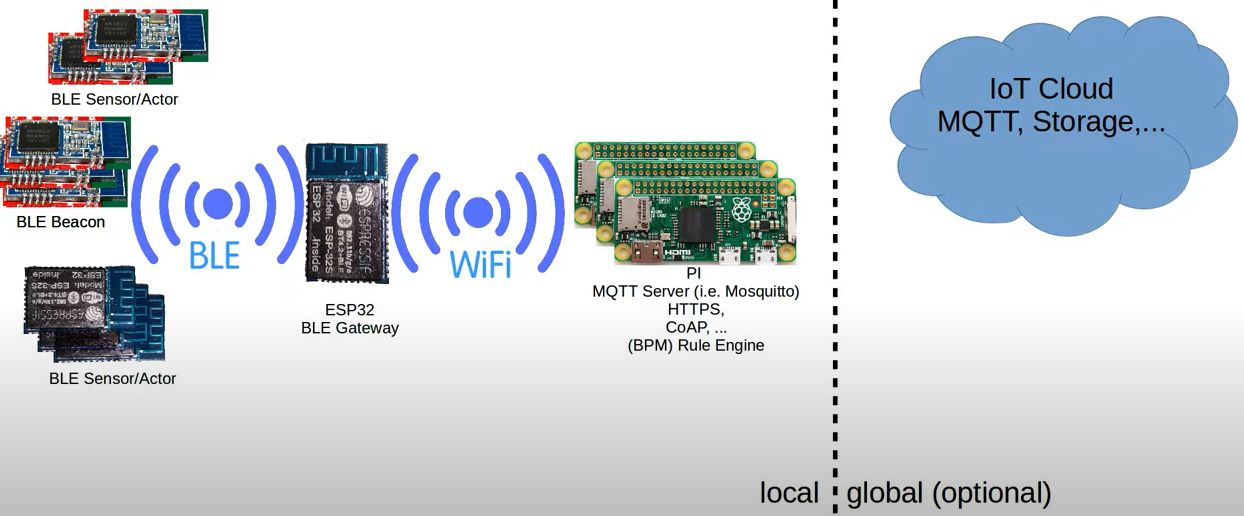
\includegraphics[width=\singlephoto]{03/01_espressif_gateway.png}  
  }
  \caption{Sistem interconectare actori Espressif la internet \cite{StackOverflow2021Espressif}}
\end{figure}

Din perspectiva utilizatorului, dispozitivele noi necesita un pas de imperechere in retea, dupa acest pas fiind complet autonome. Chiar daca frameworkul ofera functii ajutatoare pentru criptarea informatiilor transmise, aplicatiile pot alege sa implementeze metoda standard Curve25519, sa isi implementeze propriul mecanism sau chiar sa il dezactiveze complet.

Compania din spate ofera printre altele si o familie de microcontrollere numita ESP, gandita pentru a accelera procesul de dezvoltare a noi senzori si actori in retea, oferind o gama larga in materie de conectivitate.

\subsection {Solutia hobbyista}

Proiectandu-ne propriul sistem, beneficiem de libertate in modelarea problemei si alegerea protocoalelor de comunicare. Asadar, se poate concepe un sistem \acrshort{iot} care sa ofere un set de functionalitati mai restrans, folosind hardware disponibil consumatorilor de rand si tehnologii software open-source.

Aditional, pentru o integrare minimala cu unul din asistentii personali mentionati mai sus, de obicei este pus la dispozitia dezvoltatorilor un API bazat pe webhook-uri. Acesta sarcina presupune implementarea unor servicii \acrshort{rest} pe baza unor specificiatii prestabilite. 

\section {Prezentarea tehnologiilor si platformelor de dezvoltare alese}

\subsection {Hardware}

Deoarece proiectul necesita atat interactiunea cu sisteme electrice cat si cu sisteme digitale precum stiva \acrshort{ip}, am ales placa de dezvoltare "Raspberry Pi 3 Model B Rev 1.2". Aceasta ofera un procesor quad core cu arhitectura armv7 de 1.2 Ghz, 1 GB RAM si 26 de pini \acrfull{gpio} pentru interactiunea cu terminalul \acrshort{pots}.

Considerand complexitatea relativ scazuta a circuitului electric, pentru proiectarea \acrshort{pcb} am ales Fritzing, un soft open-source de \acrfull{cad}. Spre deosebire de un program mai profesionist precum Eagle, Fritzing este usor de folosit si dispune de o librarie care contine majoritatea componentelor anologice si digitale. In cazul in care nu exista model pentru o componenta, utilizatorul are posibilitatea de a crea un model din poze si masuratori. 

\subsection {Backend}

Intr-un studiu anual realizat de Stack Overflow, peste 80,000 de dezvoltatori software au ales JavaScript ca cel mai folosit limbaj de programare pentru al noualea an consecutiv. NodeJS a urcat pe locul 5 in popularitate, in timp ce Typescript este pe locul 6. Datorita cerintei de portabilitate am ales NodeJS ca limbaj pentru implementarea serverului aplicatiei. \cite{StackOverflow2021Survey}

Printre alternative viabile pentru acest tip de proiect se numara Java, C\# sau Python, limbaje aflate in primele 10 in topul celor de la Stack Overflow.

Ca framework de dezvoltare a serverului am ales NestJS, oferind o arhitectura \acrfull{mvc} si multe functionalitati convenabile precum:

\begin{itemize}
  \item Framework de injectare a dependintelor: graful (aciclic) de dependinte al aplicatiei este calculat la pornire, fiecarui modul ii sunt satisfacute dependintele, instantiindu-se obiectele necesare o singura data. Daca sunt detectati cicli in graful de dependinte sau nu exista informatii despre cum se poate instantia o clasa, atunci se va arunca o eroare de runtime si aplicatia va iesi cu un status code de eroare. 
  \item Separarea logicii de control a aplicatiei de interfata si de date. Utilizatorul interactioneaza cu interfata, care notifica controllerul de actiunile utilizatorului, controllerul executa logica aplicatiei si actualizeaza modelul corespunzator, schimbari ce se vor reflecta in interfata.
  \item Imbina elemente de \acrfull{oop}, \acrfull{fp} si \acrfull{frp}. De exemplu: modulele si serviciile sunt clase, iar decoratorii claselor sunt functii care modifica comportamentul functiilor adnotate prin compunere.

\end{itemize}

\subsection {Baza de date}

Din punct de vedere al scalabilitatii, pradigma relationala scaleaza vartical (putine servere puternice), pe cand cea nerelationala este orizontala (multe servere mici). Prin urmare am ales MongoDB, o solutie de tip NoSQL rulata in modul "cluster" pentru a oferi redundanta datelor prin replicarea lor de 3 ori pe noduri diferite fizic.

Deoarece MongoDB are nevoie de suport pentru 64 biti, nu poate fi instalata pe acelasi Raspberry Pi unde va rula si serverul. Pentru simplitudine, am ales un serviciu online de hosting gratis, numit Mongo Atlas. Asadar, serverul NodeJS trebuie sa tina cont de eventuala latenta mai ridicata in comunicarea cu baza de date si retransmiterea comenzilor in cazul in care niciunul din nodurile clusterului nu este disponibil.

\subsubsection {Object Document Mapping}

Pentru transformarea si validarea obiectelor de JavaScript in documente ce vor fi stocate in baza de date, am ales Mongoose.

\subsection {Client}

Android este o platforma mobile care s-a maturizat pe parcusul a 12 versiuni majore si principalul competitor de piata al iOS. Avand experienta anterioara ca programator Android si in special cu limbajul de programare Java, a fost o alegere convenabila pentru un prototip rapid.
Este de mentionat ca aceasta alegere de platforma este pur subiectiva, un client similar putand fi dezvoltat pentru iOS sau cu o tehnologie care suporta cross-compilation cum ar fi React Native sau Ionic.


\chapter{Considerente legate de implementarea soluției tehnice}
\section {Arhitectura sistemului}

Sistemul prezentat presupune atat o partare hardware, cat si una software. Hardwareul realizeaza adaptarea dintre terminalul analog POTS si placa digitala de dezvoltare Raspberry Pi, iar ca software am folosit NodeJS pentru server si Android pentru a implementa un client al serverului

\subsection {Raspberry Pi HUT}

Pentru a proiecta un \acrfull{pcb} am folosit softwareul Fritzing. Acesta permite proiectarea schemei electrice si ulterior trasarea conexiunilor pe layoutul fizic al placii.

Actionarea butoanelor terminalului \acrshort{pots} se realizeaza cu ajutorul unor opto-cuploare, izoland circuitul interfonului care este proiectat pentru a functiona cu spike-uri de pana la 90V de circuitul Raspberry Pi.

Detectarea unui apel este realizata prin legarea unui \acrfull{mosfet} la bornele difuzorului terminalului \acrshort{pots} si inserierea cu un amplificator operational in regim de comparator cu referinta de 0.1V. Am folosit de asemenea si un Filtru Trece Jos deoarece terminalul este sensibil la zgomote, declansand accidental notificarea.

\subsection {Webserver NodeJS}

NodeJS este un

\subsection {Android}

Android este o platforma mobile care s-a maturizat pe parcusul a 12 versiuni majore si principalul competitor de piata al iOS.


\section {Implementarea sistemului}


\section {Testarea sistemului}

\chapter{Studiu de caz}
\section{Oferirea accesului unui utilizator}

\begin{figure}[H]
\begin{center}
  \subfloat[In cazul in care aplicatia este pornita, utilizatorul este redirectat in IncomingActivity]{\label{fig:useraddga}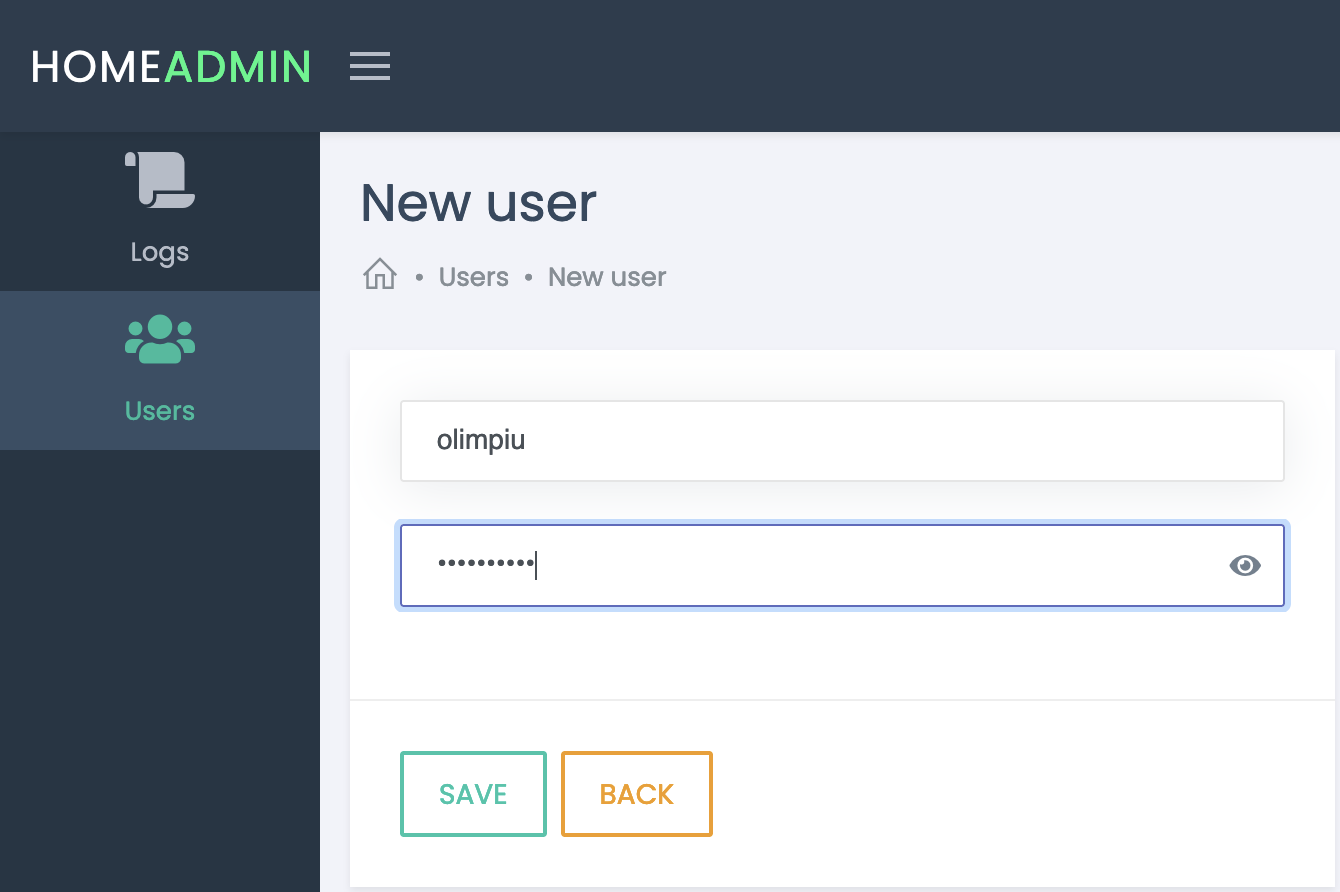
\includegraphics[width=\doublefigure]{05/06_admin_add_user.png}}
  \hfil
  \subfloat[In cazul in care aplicatia nu este in foreground, se trimite o notificare de sistem cu doua actiuni]{\label{fig:useraddgb}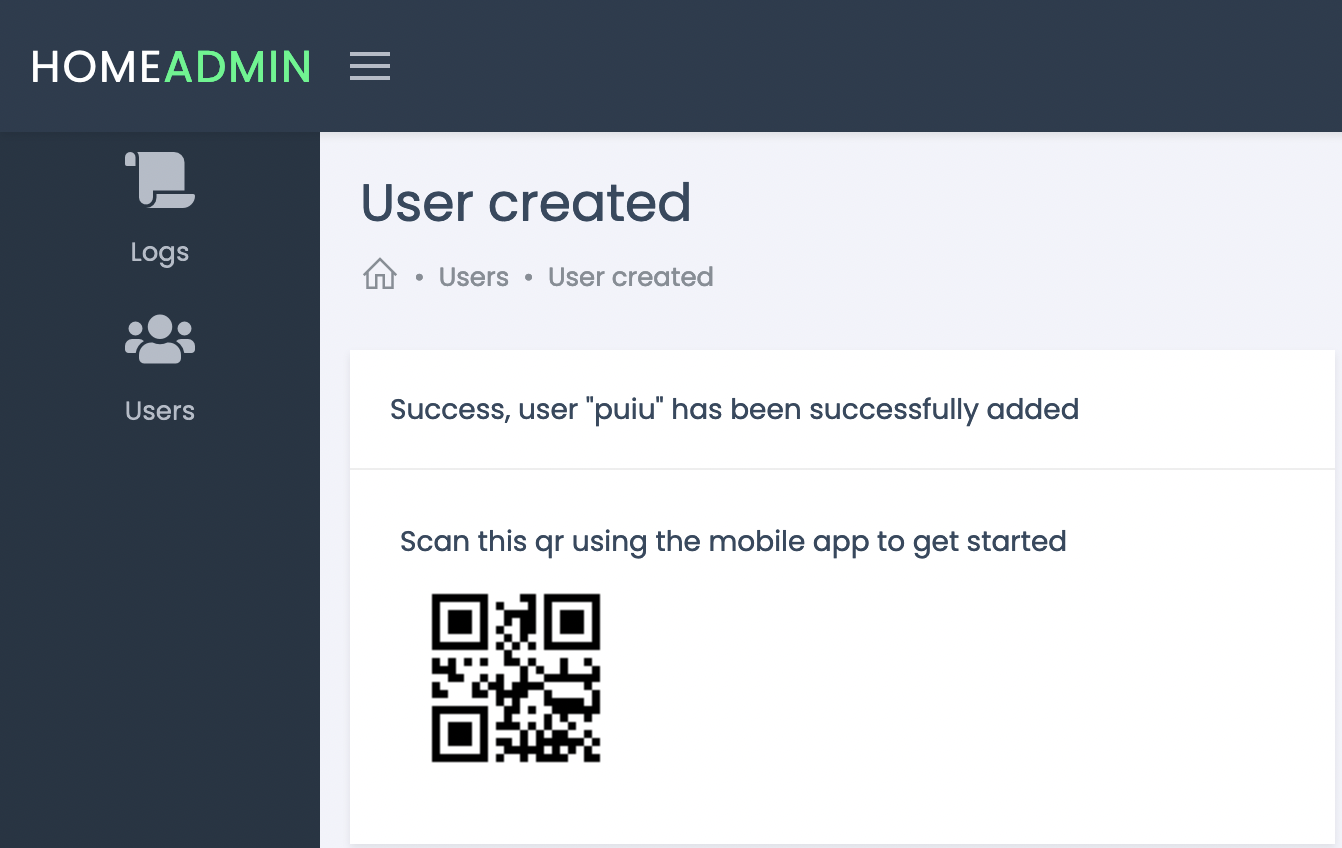
\includegraphics[width=\doublefigure]{05/07_admin_add_user_success.png}}
  \caption{Ecran apel}
  \label{fig:useraddg}
\end{center}
\end{figure}


\section{Raspuns automat}

Mi-am comandat pizza si ajunge in timp ce folosesc pistolul de lipit. Prin urmare voi programa interfonul sa raspunda si sa deschida automat usa la urmatorul apel.

\begin{figure}[H]
\begin{center}
  \subfloat[Apasarea butonului albastru auto-answer va arata meniul pentru configurarea functionalitatii]{\label{fig:autoanswera}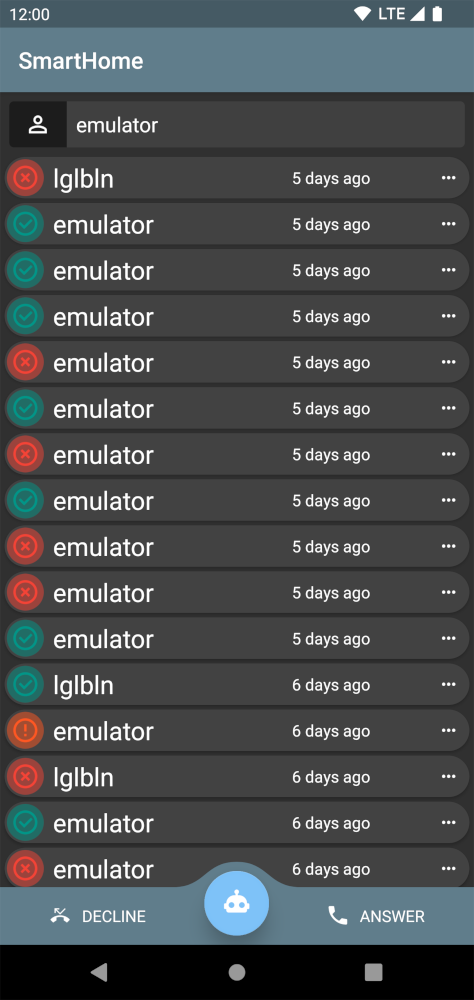
\includegraphics[width=\doublefigure]{05/01_android_autoanswer.png}}
  \hfil
  \subfloat[Alegerea unui interval pentru care functia va fi activa]{\label{fig:autoanswerb}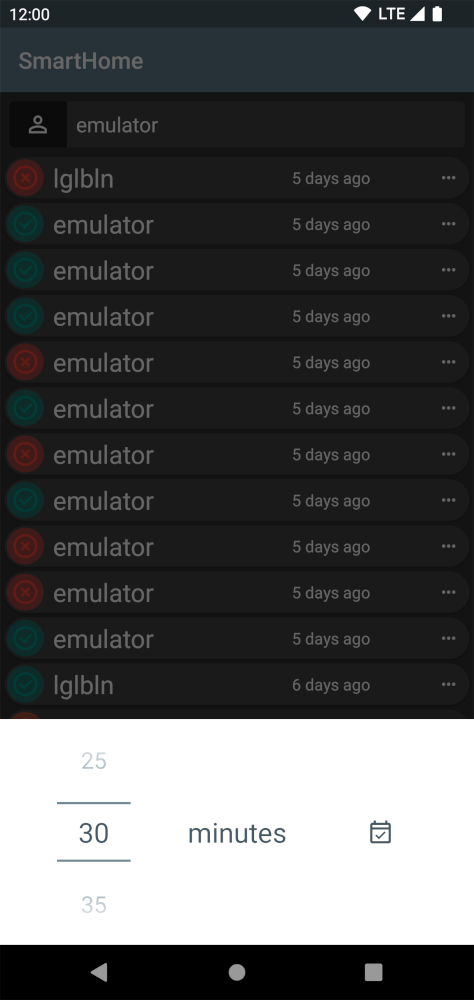
\includegraphics[width=\doublefigure]{05/02_android_auto_set.png}}
  \caption{Pasi pentru setare functie auto-answer}
  \label{fig:autoanswer}
\end{center}
\end{figure}

Se confirma ca functia este activata prin colorarea butonului auto-answer in portocaliu. Intr-o maniera similiara, daca se doreste oprirea inainte de termen, se poate face acest lucru din meniul anterior.

\section{Raspuns de la distanta}

Mi-am pierdut cartela standard \acrfull{rfid} pentru a intra in bloc. Asadar, voi suna la numerul apartamentului meu si voi folosi aplicatia mobila pentru a raspunde la propriul apel.

\begin{figure}[H]
\begin{center}
  \subfloat[In cazul in care aplicatia este pornita, utilizatorul este redirectat in IncomingActivity]{\label{fig:ringinga}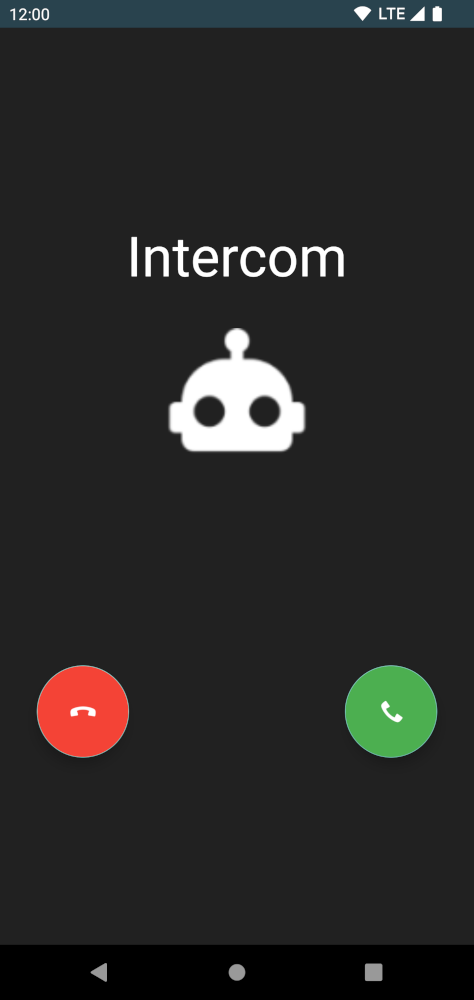
\includegraphics[width=\doublefigure]{05/04_android_app_ringing.png}}
  \hfil
  \subfloat[In cazul in care aplicatia nu este in foreground, se trimite o notificare de sistem cu doua actiuni]{\label{fig:ringingb}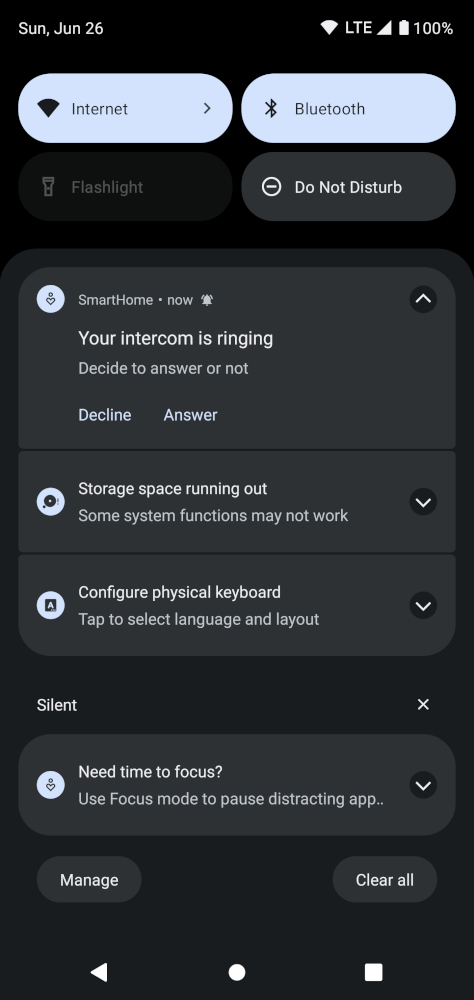
\includegraphics[width=\doublefigure]{05/05_android_notification_ringing.png}}
  \caption{Ecran apel}
  \label{fig:ringing}
\end{center}
\end{figure}

O alta varianta pentru mitigarea acestei probleme a fost folosirea unui tag \acrfull{nfc} care contine codat url-ul de acces impreuna cu un token care nu expira. Astfel prin scanarea lui cu un telefon ce dispune de anena \acrshort{nfc} se va realiza request-ul din browserul default al utilizatorului, rezultand in deschiderea interfonului.

\chapter{Concluzii}
\section{Concluzii}

Având în vedere informa'tiile expuse în capitolele 1, 2, 3 'si cuno'stin'tele dobândite în realizarea arhitecturii unui sistem de tip încuietoare inteligentă, dar 'si rezultatele studiului de caz demonstrează că se pot crea solu'tii folosind tehnologii open-source. Prin alegeri sensibile din punct de vedere tehnic în ceea ce prive'ste securitatea sistemului, utilizatorul normal poate folosi aplica'tia pentru a î'si controla interfonul într-un mod sigur. De asemenea, includerea tehnologiilor open-source înseamnă că utilizatorii avansa'ti au multiple alegeri în ceea ce prive'ste implementarea solu'tiei (pot alege unde sunt stocate datele 'si cine are acces la ele, pot configura din firewall accesul la \acrshort{api} 'si la interfa'ta administrativă).

Prin urmare, această lucrare arată că se poate concepe o solu'tie \acrshort{iot} la nivelul standardelor secolului 21, atât din punct de vedere al securită'tii cât 'si al proprietă'tii datelor stocate. Integrarea sa u'soară poate doar să beneficieze adoptării mai rapide a acestui sistem.

\section{Contribu'tii}

\begin{itemize}
  \item Sinteza informa'tiilor în ceea ce prive'ste ni'sa încuietorilor inteligente.
  \item Analiza solu'tiilor existente din domeniu pentru în'telegerea pie'tei.
  \item Conceperea arhitecturii unui sistem similar care să satisfacă cerin'tele func'tionale.
  \item S-a demonstrat că se pot folosi componente electronice simple pentru a realiza un optocuplor mai ieftin, dar care oferă acceasi func'tionalitate în cazul acestei aplica'tii.
  \item Implementarea fizica a acestui concept 'si testarea în via'tă de zi cu zi.
\end{itemize}

\section{Dezvoltări ulterioare}

Dezvoltări ulterioare ale sistemului ar presupune construirea unui terminal \acrshort{pots} întreg ca \acrshort{hat} pentru RaspberryPi. Astfel vom putea atinge 'si cerin'ta de a oferi utilizatorului fluxuri audio pentru a comunica cu persoana de la celălalt capăt al interfonului. 

%%%%%%%%%%%%%%%%%%%%%% back matter %%%%%%%%%%%%%%%%%%%%%%%%%%%%%%%%%%%%%%
% \appendix
% \appendixpage
% \addappheadtotoc
% \begin{appendices}                                          % from here onwards are the appendices
% \input{\chapters/surse}
% \end{appendices}

\cleardoublepage

\printbibliography[heading=bibintoc]
\end{document}